\documentclass[letterpaper]{article} % DO NOT CHANGE THIS
\usepackage{aaai2026}  % DO NOT CHANGE THIS
\usepackage{times}  % DO NOT CHANGE THIS
\usepackage{helvet}  % DO NOT CHANGE THIS
\usepackage{courier}  % DO NOT CHANGE THIS
\usepackage[hyphens]{url}  % DO NOT CHANGE THIS
\usepackage{graphicx} % DO NOT CHANGE THIS
\urlstyle{rm} % DO NOT CHANGE THIS
\def\UrlFont{\rm}  % DO NOT CHANGE THIS
\usepackage{natbib}  % DO NOT CHANGE THIS AND DO NOT ADD ANY OPTIONS TO IT
\usepackage{caption} % DO NOT CHANGE THIS AND DO NOT ADD ANY OPTIONS TO IT
\frenchspacing  % DO NOT CHANGE THIS
\setlength{\pdfpagewidth}{8.5in} % DO NOT CHANGE THIS
\setlength{\pdfpageheight}{11in} % DO NOT CHANGE THIS

%
% Keep the \pdfinfo as shown here. There's no need
% for you to add the /Title and /Author tags.
\pdfinfo{
/TemplateVersion (2026.1)
}

\setlength{\belowcaptionskip}{-5pt} % save space

\usepackage{amsmath, amssymb, amsthm}
\usepackage{stackengine}
\usepackage{booktabs}
\usepackage{multirow}
\usepackage{color}

\usepackage{algorithm}
\usepackage{algorithmicx}
\usepackage{algpseudocode}

\urlstyle{rm}
\def\UrlFont{\rm}


\setcounter{secnumdepth}{0} % Numbered sections



\title{Learning-Guided Simulated Annealing for the\\Capacitated Vehicle Routing Problem}

\author{
Jules Andretti,
Jérémie Cabessa,
Yann Strozecki
}

\affiliations{
David Laboratory, University of Versailles Saint-Quentin (UVSQ) – Université Paris-Saclay\\
78000 Versailles, France \smallskip\\
\{jules.andretti, jeremie.cabessa, yann.strozecki\}@uvsq.fr
}


\begin{document}

\maketitle

\begin{abstract}
The Capacitated Vehicle Routing Problem (CVRP) is a fundamental combinatorial optimization challenge with broad industrial relevance. Classical metaheuristics such as Simulated Annealing (SA) offer asymptotic convergence guarantees but suffer from inefficient random neighborhood exploration. Conversely, recent deep learning approaches generate solutions rapidly but often struggle to generalize beyond the instance sizes encountered during training. In this paper, we bridge this gap by proposing Learning-Guided Simulated Annealing (LG-SA), a hybrid framework that augments SA with a very lightweight neural module, trained to select promising neighboring solutions instead of relying on uniform sampling. The move-selection policy is learned through reinforcement learning (RL) using Proximal Policy Optimization (PPO). Through extensive experiments, we analyze the stability of the model as well as the impact of diverse feasibility mechanisms, initialization strategies, neighborhood operators, and action parameterizations (joint vs. conditional). We further show that LG-SA excels at finding high-quality solutions rapidly. In addition to achieving a 42.5\% cost reduction over classical SA and generalizing well to larger instances, LG-SA outperforms or performs on par with widely used methods like OR-Tools, attention-based GNNs, and advanced RL methods within comparable or shorter timeframes.
\end{abstract}


\section{Introduction}

Combinatorial Optimization Problems (COPs) are everywhere in real-world applications, ranging from logistics and supply chain management to network design. Among them, the Capacitated Vehicle Routing Problem (CVRP) stands as a cornerstone problem, famously known to be NP-hard \cite{dantzig_truck_1959, liu_heuristics_2023, shi_brief_2023, bogyrbayeva_learning_2022}. The objective is to determine a set of optimal routes for a fleet of vehicles to serve a set of customers under capacity constraints. Despite decades of research, finding high-quality solutions for large-scale instances in limited time remains a significant challenge.

Traditional approaches fall into two categories. \textit{Exact methods}, such as Branch-and-Cut, guarantee optimality but become computationally intractable for large instances. \textit{Heuristics and Metaheuristics}, such as Simulated Annealing (SA), Tabu Search, or Genetic Algorithms, offer a more scalable alternative by exploring the solution space stochastically. However, these methods typically rely on uniform sampling to generate candidate moves. Such ``blind'' exploration often leads to slow convergence and requires extensive, instance-specific parameter tuning to prevent stagnation in local optima.

Recently, \textit{Machine Learning (ML) for COPs} has emerged as a promising paradigm. Constructive neural approaches, such as the Attention Model (AM) \cite{kool_attention_2019}, learn to build solutions node by node. While fast, they often struggle to \textit{generalize}: a model trained on 50 nodes typically performs poorly on 500-node instances. Moreover, once a solution is constructed, these methods lack mechanisms for refinement. These limitations led to a growing interest in Neural Improvement Heuristics \cite{wu_learning_2022,garcia-torres_combining_2022}, which learn to iteratively repair or improve a complete solutions.

In this work, we propose \textit{Learning-Guided Simulated Annealing (LG-SA)}, a hybrid framework marrying the theoretical robustness of Simulated Annealing (SA) with the adaptive guidance of Deep Reinforcement Learning (DRL). Our method extends Neural Simulated Annealing (NSA) \citep{correia_neural_2023} to the more complex context of CVRP, explicitly accounting for capacity constraints that invalidate many local moves. Specifically, we augment SA by replacing random neighbor selection with a very lightweight neural policy trained via PPO. This policy learns to interpret structural features and propose ``smart'' moves to reduce cost, while the Metropolis criterion of SA preserves the ability to escape local optima.

Our main contributions are summarized as follows:
\begin{itemize}
\item We introduce LG-SA, a hybrid learning-informed metaheuristic that enhances the local search of SA with a lightweight neural policy trained via PPO. 
\item We introduce and evaluate feasibility-enforcement strategies to handle the hard constraints specific to CVRP. We demonstrate that explicitly masking invalid actions (\textit{proactive filtering}) is essential for both training stability and search performance.
\item Through extensive experiments, we analyze the stability of the model as well as the impact of diverse initialization strategies, neighborhood operators, and action parameterizations (joint vs. conditional).
\item We demonstrate that LG-SA significantly outperforms the classical SA baseline with a 42.5\% cost reduction, generalizes effectively to larger instance sizes, and outperforms or competes closely with state-of-the-art solvers and learning-based methods in both solution quality and computational efficiency \citep{ortools_routing, kool_attention_2019, nazari_reinforcement_2018}.
\end{itemize}
Overall, these results establish LG-SA as an excellent balance between fast constructive heuristics and more computationally intensive solvers or heavy learning-based methods. Finally, in an effort toward transparency and full reproducibility, we make the complete source code and experimental data publicly available at the following repository\footnote{\url{https://github.com/JAndretti/Learning-Guided-Simulated-Annealing-for-the-Capacitated-Vehicle-Routing}}.

\section{Background and Related Work}

Since its introduction by \citet{dantzig_truck_1959}, the CVRP has been tackled by exact algorithms (e.g., branch-and-cut) that struggle at scale due to NP-hardness \cite{toth_vehicle_2002}. This necessitates heuristics, ranging from basic construction methods \cite{clarke_scheduling_1964} to metaheuristics \cite{kirkpatrick_optimization_1983} and general solvers like OR-Tools \cite{ortools_routing, liu_heuristics_2023,muriyatmoko_heuristics_2024}. While many require careful tuning, state-of-the-art metaheuristics offer remarkable performance; notably, \citet{vidal_hybrid_2022} introduced a highly effective, open-source Hybrid Genetic Search (HGS) utilizing the SWAP* neighborhood, establishing a leading standard for solution quality and convergence speed.

Recent deep learning approaches typically follow construction or improvement paradigms. Constructive methods generate solutions end-to-end: \citet{nazari_reinforcement_2018} utilized reinforcement learning (RL) with attention mechanisms, while \citet{kool_attention_2019} proposed a versatile Attention Model (AM) trained via REINFORCE. Conversely, improvement methods iteratively refine solutions: \citet{wu_learning_2022} framed local search as a Markov Decision Process, and \citet{gao_learn_2020} learned destruction-repair operators for Very Large Neighborhood Search (VLNS) using Graph Attention Networks.

Hybridizing neural networks with classical heuristics has proven highly effective. \citet{garcia-torres_combining_2022} combined a deep constructor with a deep perturbator, while \citet{bui_imitation_2023} used Imitation Learning—treating classical heuristics like HGS as experts—to scale solutions up to 30{,}000 nodes. Most closely related to our work is Neural Simulated Annealing (NSA) by \citet{correia_neural_2023}, which learns proposal distributions to enhance classical SA while preserving convergence guarantees. However, NSA has not yet been applied to the CVRP, where capacity constraints heavily restrict feasible local moves.



\section{Problem Definition}
\label{Problem Definition}

The {\it Capacitated Vehicle Routing Problem (CVRP)} is defined on a complete undirected graph $G = (V, E)$, where $V = \{0\} \cup \mathcal{C}$ and $E = V \times V$ denote the sets of nodes and edges, respectively. Node $0$ corresponds to the central depot, and $\mathcal{C} = \{1, \dots, N\}$ represents the set of $N$ customers. 

Each edge $(i, j) \in E$ is associated with a non-negative travel cost $c_{ij}$ (satisfying $c_{ij} = c_{ji}$). Each customer $i \in \mathcal{C}$ has a non-negative demand $d_i$, while the depot has zero demand ($d_0 = 0$). A fleet of $K$ identical vehicles, each with uniform capacity $Q$, is stationed at the depot.

A route $R_k = (0, v_1, v_2, \ldots, v_p, 0)$ is a simple cycle (tour) starting and ending at the depot, where $\{v_1, \ldots, v_p\} \subseteq \mathcal{C}$ denotes the subset of customers served by vehicle $k$. A \textit{solution} $s = \{R_1, \ldots, R_m\}$ consists of a set of $m$ routes. A solution $s$ is considered \textit{feasible} if and only if it satisfies the following conditions:
\begin{enumerate}
    \item The number of routes does not exceed the number of available vehicles, i.e., $m \leq K$.
    \item Each customer is visited exactly once by a single vehicle,
    $$
    \sum_{k=1}^{m} \mathbf{1}_{\{i \in R_k\}} = 1, \quad \forall i \in \mathcal{C} .
    $$
    % where $\mathbf{1}_{\{i \in R_k\}}$ equals $1$ if customer $i$ belongs to route $R_k$, and $0$ otherwise.

    \item For every route $R_k$, the total demand of its customers does not exceed the vehicle capacity $Q$, i.e.,
    $$
    \sum_{i \in R_k \setminus \{0\}} d_i \leq Q, \quad \forall k = 1, \ldots, m.
    $$
\end{enumerate}
The set of \textit{feasible solutions} is denoted by $\mathcal{F}$.

Let $x_{ij}(s)$ be a binary indicator variable defined by $x_{ij}(s) = 1$ if edge $(i,j)$ is traversed in any route $R_k$ of $s$, and $x_{ij}(s) = 0$ otherwise. The objective of the CVRP is to find a feasible solution $s^* \in \mathcal{F}$ that minimizes the total travel cost $C(s)$:
$$
s^* = \arg\min_{s \in \mathcal{F}} \Big\{ C(s) = \sum_{i \in V} \sum_{j \in V, i < j} c_{ij} x_{ij}(s) \Big\}
$$



\section{Proposed Method}


\subsection{Overview}


We propose a hybrid metaheuristic combining a \textit{Simulated Annealing (SA)} process with a lightweight \textit{Neural Reinforcement Learning (RL) policy}. The SA component orchestrates the global exploration of the solution space, while the RL-trained neural network (NN) adaptively guides the selection of neighboring solutions.

\textit{Simulated Annealing} (SA) is an optimization heuristic that explores the neighborhood of a current solution in a stochastic manner. Given a solution $s$, SA samples a neighboring solution $s' \in \mathcal{N}(s)$ and accepts it according to the \textit{Metropolis criterion}: improving moves are always accepted, while worsening moves are accepted with probability $\exp(-\Delta C / T)$, where $\Delta C = C(s') - C(s)$ is the cost difference and $T$ is the temperature. This stochastic acceptance, regulated by $T$, allows to escape local optima.

In our framework, the sampling of a neighboring solution $s' \in \mathcal{N}(s)$ is no longer uniform but instead follows a probability distribution learned by a lightweight \textit{neural network (NN)}. Formally, let $H: \mathcal{S} \times \mathcal{A} \to \mathcal{S}$ denote a \textit{neighborhood operator} that, for each solution $s \in \mathcal{S}$ and possible action $a \in \mathcal{A}(s)$ on $s$, produces the neighboring solution $s' = H(s, a) \in \mathcal{S}$.
For instance, $a \in E \times E$ may represent a pair of edges, and $s' = H(s, a)$ is the solution obtained by exchanging those edges in $s$.
The neighborhood of $s$ is thus defined as
$$
\mathcal{N}(s) = \left\{ H(s, a) : a \in \mathcal{A}(s) \right\}.
$$
In classical SA, the neighboring solution $s'$ of $s$ is obtained through \textit{uniform sampling}, i.e.,
$$
a \sim \mathcal{U}(\mathcal{A}(s)) \quad \text{and} \quad s' = H(s, a) \in \mathcal{N}(s).
$$
By contrast, in our framework, a neural network policy $\pi_\theta$ learns a \textit{probability distribution} $\pi_\theta(\cdot \mid s) \in \Delta(\mathcal{A}(s))$ over the (feasible) actions on $s$, and the neighboring solution is selected according to
\begin{align*}
a \sim \pi_\theta(\cdot \mid s) \quad \text{ and } \quad s' = H(s, a) \in \mathcal{N}(s).
\end{align*}
The neural policy is learned by \textit{Reinforcement Learning (RL)} using \textit{Proximal Policy Optimization (PPO)}, as explained later in further details.

To control the temperature $T$ in SA, we evaluated several cooling schedules, including a \textit{step decay} (halving $T$ every $n$ steps) and a \textit{geometric} (or \textit{lambda}) schedule defined as
$$
T_{k+1} = \alpha \, T_k, \quad \text{with } \alpha = \left( {T_K /T_0} \right)^{1/K}.
$$
This setting ensures a consistent decay from $T_0 = 1.0$ to $T_K = 0.1$ over the $K$-step search horizon. Empirically, we noticed that simple monotonic schedules performed best, so we adopted the geometric schedule in our experiments. The overall procedure is summarized in Algorithm~\ref{alg:learning_guided_sa_conceptual}.

\begin{algorithm}[t]
\begin{algorithmic}[1]
\caption{Overview of the Learning-Guided SA}
\label{alg:learning_guided_sa_conceptual}
\Require Initial solution $s$, learned neural policy $\pi_\theta$, neighborhood operator $H$
\State Initialize $s^*$ and SA parameters (e.g., $T$)

\While{SA termination criterion not met}
    \State \textit{1. Model-Guided Neighbor Generation}
    \State \quad Encode current solution $s$
    \State \quad Sample action from policy: $a \sim \pi_\theta(a \mid s)$
    \State \quad Generate candidate solution: $s' \gets H(s, a)$
    
    \State \textit{2. Standard SA Procedure}
    \State \quad $s \gets \text{SA\_accept}(s, s', T)$ 
    \State \quad Update $T$ and $s^*$
\EndWhile

\State \Return $s^*$
\end{algorithmic}
\end{algorithm}


\subsection{Neural Model}
\label{Neural Model}

\paragraph{Generalities.}

The \textit{neural model} guides the selection of neighboring solutions. Given a current solution $s$, it assigns a score $z_{ij}$ to each candidate pair of customers (nodes) $(i, j)$. This score reflects the estimated likelihood that modifying $s$ through the pair $(i, j)$ will yield an improved solution $s'$. An action $a = (i, j)$ is then sampled according to the probability distribution induced by the scores $z_{ij}$, and the neighboring solution is obtained as $s' = H(s, a)$. The neural model is illustrated in Figure~\ref{fig_LGSA}.

\begin{figure}[t]
\centering
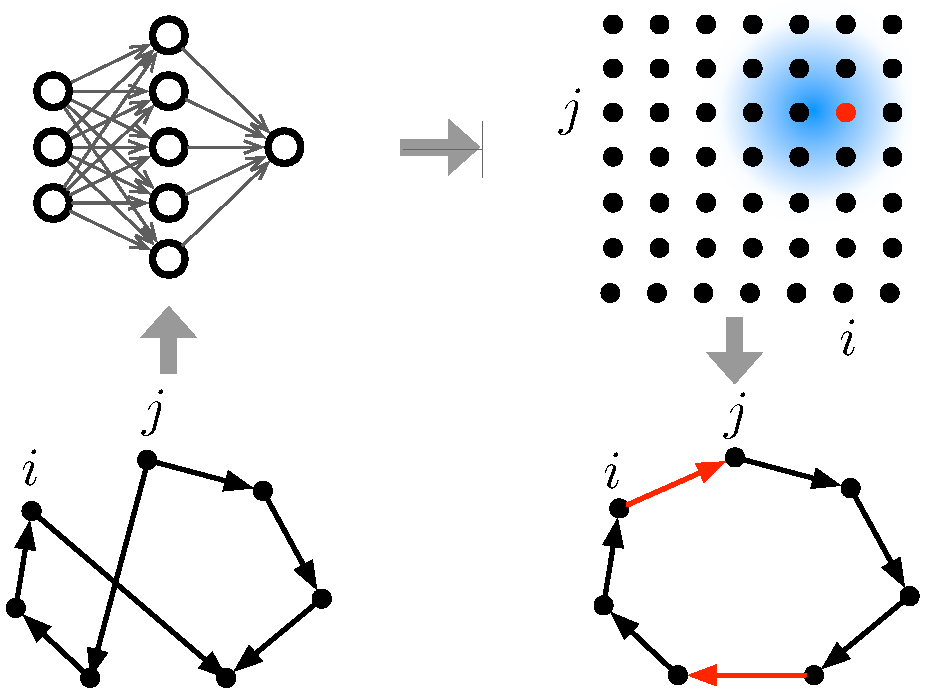
\includegraphics[width=6.2cm]{LGSA.pdf}
\caption{All nodes of the current solution $s$ are encoded and fed to the lightweight neural network -- either in a direct (joint) manner ($N^2$ node pairs) or in a two-stage (conditional) manner ($2N$ nodes). The output scores of the network produce a distribution over all node pairs. A pair $a=(i,j)$ is then sampled from this distribution, which yields the neighboring solution $s' = H(s,a)$.}
\label{fig_LGSA}
\end{figure}


\paragraph{Neighborhood operators.}

We consider three standard neighborhood operators defined over a pair of nodes $(i, j)$. In our framework, the operator is fixed: each experiment uses a single operator $H$ during both training and testing. The neural policy is therefore trained to learn a distribution tailored to that operator. The available operators are:

\begin{itemize}
    \item \textit{Swap:} Exchanges the positions of nodes $i$ and $j$, either within the same route or across different routes.
    \item \textit{Insertion (Relocation):} Removes node $i$ from its current position and reinserts it immediately after node $j$.
    \item \textit{2-opt:} Reverses a segment of the tour by removing edges $(i,\text{succ}(i))$ and $(j,\text{succ}(j))$ and reconnecting the tour after reversing the path from $\text{succ}(i)$ to $j$.
\end{itemize}


\paragraph{Input representation.}

We consider two-dimensional (2D) CVRP instances with coordinates normalized to $[0, 1]$. To ensure \textit{scale invariance} and applicability to any problem size $N$, we utilize a \textit{node-centric} representation where each client $i$ is encoded via a local feature vector $\mathbf{x}_i$, avoiding fixed-size global descriptors. Formally, $\mathbf{x}_i$ incorporates the following spatial, positional, and capacity-related features:
\begin{equation*}
    \mathbf{x}_i =
    \big[
        \mathbf{p}_i,\, \mathbf{p}_{\text{depot}},\,
        \mathbf{p}_{\text{neigh}(i)},\,
        \mathbf{1}_{\{i=0\}},\,
        \theta_i,\, d_{i0},\,
        \tfrac{q_i}{Q_{\text{route}}},\,
        \tfrac{Q_{\text{route}}}{Q},\,
        \tfrac{q_i}{Q}
    \big],
\end{equation*}
Here, $\mathbf{p}_{(\cdot)}$ denotes the coordinates (of node $i$, the depot, and its neighbors in solution $s$), $\mathbf{1}_{\{i=0\}}$ is a depot flag, and $\theta_i, d_{i0}$ are relative polar and radial positions. Node and route demands, normalized by vehicle capacity $Q$, are given by $q_i$ and $Q_{\text{route}}$. The feature vector also includes the Simulated Annealing (SA) temperature $T$ and normalized remaining steps to track optimization progress.

\paragraph{Neural architectures for action selection.}
\label{par:neural_architectures}
We investigate two lightweight architectures to model the probabilistic selection of a node pair $(i, j)$:

\begin{enumerate}
    \item \textit{Two-stage (Conditional):} 
    This architecture decomposes the selection into two sequential steps using distinct simple MLPs. First, a network $f_{\theta}$ computes a score $z_i = f_{\theta}(\mathbf{x}_i)$ for each node, and a first node $i$ is sampled via:
    $$
    i \sim P(\cdot) = \mathrm{softmax} \big( \{ z_i : i \in \mathcal{C} \} \big).
    $$
    Next, the feature vector $\mathbf{x}_i$ of the selected node is concatenated with that of every other node $j$. A second network $g_{\theta}$ assigns a score $z_{ij} = g_{\theta}(\mathbf{x}_i \oplus \mathbf{x}_j)$ to each candidate pair, and $j$ is sampled from the conditional distribution:
    $$
    j \sim P(\cdot \mid i) = \mathrm{softmax} \big( \{ z_{ij} :  j \in \mathcal{C} \} \big).
    $$
    This effectively factorizes the joint probability as $P(i, j) = P(i) \times P(j \mid i)$. Since the second network is only evaluated for the selected node $i$, this approach scales linearly with the problem size, i.e., $O(N)$.
    \item \textit{Direct (Joint):} 
    Alternatively, a single MLP $f_{\theta}$ directly processes all possible pairs to compute scores $z_{ij} = f_{\theta}(\mathbf{x}_i \oplus \mathbf{x}_j)$. The pair $(i, j)$ is then sampled in a single step from the joint distribution:
    $$
    (i, j) \sim P(\cdot, \cdot) = \mathrm{softmax} \big( \{ z_{ij} : i,j \in \mathcal{C} \} \big).
    $$
    Unlike the conditional approach, this formulation captures the compatibility of nodes $i$ and $j$ simultaneously. However, it requires evaluating all node pairs, resulting in a quadratic computational cost of $O(N^2)$.
\end{enumerate}

Both strategies define a stochastic policy $\pi_\theta(a \mid s)$ over the action space $\mathcal{A} = \mathcal{C} \times \mathcal{C}$. An action $a = (i, j)$ is sampled from this policy to generate the next solution $s'$ via the neighborhood operator $H$:
\begin{equation}
    a \sim \pi_\theta(\cdot \mid s) \quad \text{ and } \quad s' = H(s, a). \label{eq:nhood_selection}
\end{equation}


\subsection{Feasibility Strategies}


In practice, many potential actions $a$ can produce a neighboring solution $s' = H(s, a)$ which are not feasible, often by violating the vehicle-capacity constraint $C$. To address this important issue, we propose three strategies which ensure that the search process remains within the space of feasible solutions $\mathcal{F}$.

\paragraph{Proactive feasibility filtering (action masking).} 
Let $\mathcal{A}(s)$ denote the set of all actions applicable to solution $s$ under the neighborhood operator $H$.
This strategy first identifies the subset of feasible actions
\begin{equation*}
\mathcal{A}_f(s) = \{ a \in \mathcal{A}(s) \mid H(s, a) \in \mathcal{F} \}.
\end{equation*}
The policy network $\pi_\theta$ is then restricted to sample actions exclusively from this feasible subset:
\begin{equation*}
a \sim \pi_\theta(\cdot \mid s, a \in \mathcal{A}_f(s)).
\end{equation*}
In practice, this is implemented by masking all infeasible actions $a \notin \mathcal{A}_f(s)$ with zero probability. This guarantees that every accepted move yields a feasible neighbor $s' = H(s, a) \in \mathcal{F}$, but at the cost of a non-negligible computational overhead, as $\mathcal{A}_f(s)$ must be recomputed at each decision step.

\paragraph{Reactive rejection.} 
To avoid the overhead of explicit filtering, this simpler strategy allows the policy $\pi_\theta$ to select any action $a \in \mathcal{A}(s)$ according to its learned distribution. The resulting solution $s' = H(s, a)$ is then checked for feasibility. 
If $s' \notin \mathcal{F}$, the move is rejected and the current solution $s$ is retained for the next iteration. While computationally cheaper, this approach can be inefficient, as many sampled moves may be infeasible and yield no learning signal.

\paragraph{Indirect representation with greedy reconstruction.}
This strategy allows the policy to operate on unconstrained customer permutations, with feasibility enforced afterward via a reconstruction heuristic.
\begin{enumerate}
    \item The current feasible solution $s$, encoded as a single sequence (e.g., $[0,2,5,7,0,1,4,3,6,0]$), is mapped to an unconstrained permutation $s_p$ of the $N$ customers (e.g., $s_p = \langle 2,5,7,1,4,3,6 \rangle$).
    \item The neural network operates in this permutation space, producing a modified permutation $s'_p$ (e.g., $s'_p = \langle 2,5,1,7,4,3,6 \rangle$).
    \item A deterministic reconstruction heuristic $h$ then maps $s'_p$ back to a feasible solution $s' = h(s'_p) \in \mathcal{F}$.
    Typically, $h$ is a \textit{greedy split} algorithm that packs customers from $s'_p$ into routes until capacity $C$ is reached (e.g., $s' = [0,2,5,0,1,7,4,3,6,0]$).
\end{enumerate}

This approach guarantees $s' \in \mathcal{F}$ by construction and frees the policy $\pi_\theta$ from handling feasibility. However, search efficiency depends strongly on the reconstruction heuristic $h$. Although optimal split algorithms exist \cite{vidal_technical_2016}, they are far more computationally expensive than greedy variants. Because reconstruction occurs at every search step, this cost becomes prohibitive for both training and inference, especially as problem size grows.

\subsection{Reinforcement Learning with PPO}
\label{sec:reinforcement_learning}

We frame the iterative improvement process as a Markov Decision Process (MDP). At step $t$, the agent observes the current solution state $s_t$ and samples an action $a_t$ (a pair of nodes) from a policy $\pi_\theta$. The transition to the next state $s_{t+1} = H(s_t, a_t)$ yields a reward $r_t$ proportional to the improvement in solution quality.

To maximize cumulative rewards, we employ \textit{Proximal Policy Optimization (PPO)} \cite{schulman_proximal_2017}, a state-of-the-art on-policy gradient method. PPO relies on an \textit{Actor-Critic} architecture to stabilize learning:
\begin{itemize}
    \item \textbf{Actor} ($\pi_{\theta}(a_t \mid s_t)$): A network parameterized by $\theta$ that outputs a probability distribution over feasible actions.
    \item \textbf{Critic} ($V_{\phi}(s_t)$): A network parameterized by $\phi$ that estimates the value of the current solution, serving as a baseline to reduce the variance of gradient updates.
\end{itemize}

The key feature of PPO is its mechanism to enforce a \emph{trust region} constraint. To prevent destructive updates, where the new policy deviates excessively from the old one, PPO maximizes a \emph{clipped surrogate objective}. Let $\rho_t(\theta) = \frac{\pi_{\theta}(a_t \mid s_t)}{\pi_{\theta_{\text{old}}}(a_t \mid s_t)}$ be the probability ratio between the new and old policies. The objective is defined as:
\begin{equation*}
    L^{\text{CLIP}}(\theta) = \hat{\mathbb{E}}_t \Big[ \min \big( \rho_t(\theta) \hat{A}_t, \ \text{clip}(\rho_t(\theta), 1 - \epsilon, 1 + \epsilon) \hat{A}_t \big) \Big],
\end{equation*}
where $\hat{A}_t$ is the advantage function, measuring how much better an action was than expected, and $\epsilon$ is a hyperparameter (e.g., $0.2$). The clipping term removes the incentive for the probability ratio to move outside the interval $[1 - \epsilon, 1 + \epsilon]$, ensuring that policy updates remain conservative and stable.

In our implementation, the Actor and Critic are instantiated as distinct networks (no shared parameters) to prevent feature interference. They are trained concurrently: the Actor maximizes $L^{\text{CLIP}}$, while the Critic minimizes the mean-squared error between its value predictions and the observed returns.


\paragraph{Reward.}

A standard reward for CVRP is the direct cost improvement, $r_t = C(s_t) - C(s_{t+1})$ \citep{correia_neural_2023}. However, this signal is misaligned with our PPO-SA framework, as it fails to distinguish between different types of failed actions: an \textit{invalid move} (a policy error) versus a \textit{valid-but-rejected move} (a stochastic SA outcome).

We therefore design a reward $r_t$ that provides a precise signal for each case. First, we define a normalization function which scales any non-zero cost improvement $I_t = C(s_t)-C(s_{t+1})$ relative to the initial solution cost $C(s_0)$. This prevents large cost changes from dominating the reward signal:
\begin{equation*}
    \text{normalize}(I_t) = \text{clip} \Big[ \frac{I_t / C(s_0)}{R_{\text{scale}}}, -1, 1 \Big] ,
\label{eq:reward_norm}
\end{equation*}
where we use a typical scale of $R_{\text{scale}} = 0.2$.

Our reward $r_t$ is then defined by a hierarchy based on the action's outcome. If the proposed action $a_t$ is invalid (e.g., violates hard capacity constraints), it is immediately rejected, and the policy is strongly penalized: $r_t = -1.5$. If the action is valid but rejected by the SA Metropolis criterion ($I_t = 0$), this is a neutral outcome: $r_t = 0$. Finally, if the action is valid and accepted ($I_t \neq 0$), the normalized reward is used: $r_t = \text{normalize}(I_t)$. 

This tiered design is critical: it teaches the policy to avoid invalid moves (the -1.5 penalty), while remaining neutral on stochastic rejections (the 0 reward), and seeking accepted moves (the normalized reward). It separates the learning of hard constraints from the learning of solution quality.



\paragraph{Exploration.}

In standard RL applications, policies are often exploited \textit{greedily} by selecting the $a_t$ action with highest probability, i.e.,
$$
a_t = \arg \max_{a \in \mathcal{A}(s_t)} \pi_{\theta}(a \mid s_t) \,.
$$
Our framework deviates from this standard. As the PPO agent acts as a move generator for a SA step, we retain stochastic sampling even during exploitation. Formally, the action $a_t$ is sampled as
\begin{equation*}
a_t \sim \pi_{\theta}(\cdot \mid s_t),
\end{equation*}
which then produces the neighboring solution $s_{t+1} = H(s_t, a_t)$. 
Keeping this stochastic selection process is crucial: a greedy policy would repeatedly propose only the ``best'' move, limiting exploration and undermining SA's ability to escape local optima. By sampling from the policy distribution, we provide SA with a diverse set of candidate moves, letting its acceptance criterion naturally balance \textit{exploration} and \textit{exploitation}.



\section{Experimental Results}

\subsection{Evaluation Protocol}

We evaluate our approach on two widely used CVRP instance generation schemes. The first follows the setting of \cite{nazari_reinforcement_2018}, where depot and customer coordinates are sampled uniformly in the unit square $[0,1]\times[0,1]$, and customer demands are drawn uniformly from $\{1,\ldots,9\}$. 

The second scheme utilizes the large-scale dataset of \cite{queiroga_10000_nodate}, an extension of the benchmark suite by \cite{uchoa_new_2017}, specifically designed for assessing learning-based CVRP methods. This dataset contains 10{,}000 Euclidean instances with 100 customers and exhibits wide structural diversity. Instances feature varying spatial organizations -- including \textit{sparse}, \textit{highly concentrated}, and \textit{clustered} distributions -- as well as multiple demand patterns and average route densities. Nearly all instances are accompanied by optimal solutions computed using exact solvers.

All computational experiments and runtime measurements were conducted on a single machine equipped with an AMD Ryzen 9 9900X CPU and an NVIDIA RTX 5070 GPU. Under this setup, the training time for a single model is approximately 40 minutes. 


\subsection{Parameter Analysis}

In this section, we analyze the contribution of the different components of our architecture as well as the impact of key parameters. Unless stated otherwise, all experiments are conducted on a batch of $1{,}000$ uniform CVRP instances generated following the distribution of \citet{nazari_reinforcement_2018}, with $N = 100$ customers and vehicle capacity $50$. Each search process is executed for $10{,}000$ steps, starting from a randomly generated initial solution. Crucially, to leverage the full capability of our neural architecture, all $1{,}000$ instances are solved in parallel on a single GPU.



\paragraph{Stability Analysis.}
We assess the stability of our approach from two perspectives: the reproducibility of the training process and the robustness of the stochastic search during inference.

\textit{Training Stability.} To evaluate the consistency of the learning procedure, we trained the model 15 times with different seeds and evaluated each one. The mean and median costs are $17.53$ and $17.60$, respectively, with a best–worst gap of $1.78\%$ ($17.41$ vs.\ $17.72$), indicating stable performance across runs.

\textit{Inference Stability.} We further analyzed the robustness of the search process on a single test instance, solved $10{,}000$ times starting from different random initial solutions. Our model ($10{,}000$ steps) was compared against the random baseline ($200{,}000$ steps). The model achieved a mean cost of $16.29$ with a standard deviation of $0.19$, whereas the baseline averaged $23.80$ with a significantly higher standard deviation of $0.42$.
This reduced variance ($0.19$ vs $0.42$) demonstrates that the learned policy consistently guides the search toward similar local minima regardless of the starting point. In contrast, the baseline yields widely varying results dependent on the stochasticity of the random walk.


\paragraph{Feasibility enforcement and Metropolis criterion.} 

We evaluate how the three feasibility-enforcement strategies -- \textit{proactive filtering}, \textit{reactive rejection}, and \textit{indirect representation} -- interact with the Metropolis acceptance criterion. Table~\ref{tab:feasibility_metropolis} reports the final costs and runtimes under short (1k steps) and medium (10k steps) search horizons.

\begin{table}[t]
\centering
\small
\setlength{\tabcolsep}{4pt}
\begin{tabular}{cc cccc}
\toprule
& & \multicolumn{2}{c}{1{,}000 steps} & \multicolumn{2}{c}{10{,}000 steps} \\
\cmidrule(lr){3-4} \cmidrule(lr){5-6}
%\shortstack{Update \\ Method} 
Feasibility & Metropolis & Cost & Time (s) & Cost & Time (s) \\
\midrule
\multirow{2}{*}{\shortstack{Proactive \\ Filtering}} 
 & False & 19.25 & 2.24 & 17.72 & 22.11 \\
 & True  & \textbf{18.92} & 2.38  & \textbf{17.39} & 23.36 \\
%\cmidrule(lr){2-6}
\midrule
\multirow{2}{*}{\shortstack{Reactive \\ Rejection}} 
 & False & 23.73 & 2.15  & 22.47 & 20.78 \\
 & True  & 23.60 & 2.14  & 21.66 & 20.80 \\
%\cmidrule(lr){2-6}
\midrule
\multirow{2}{*}{\shortstack{Indirect \\ Rep.}} 
 & False & 20.46 & 8.77  & 19.15 & 91.13 \\
 & True  & 20.10 & 9.15  & 18.15 & 92.41 \\
\bottomrule
\end{tabular}
\caption{Impact of feasibility strategies and Metropolis criterion (1k vs 10k steps). Costs are averaged over the test set.}
\label{tab:feasibility_metropolis}
\end{table}

We observe that enabling the Metropolis acceptance criterion improves performance across \textit{all} feasibility-enforcement strategies. For example, with a 10k-step horizon, \textit{indirect representation} improves from 19.15 to 18.15, and \textit{proactive filtering} from 17.72 to 17.39. This uniform benefit confirms that the policy primarily serves as an effective move generator, while the Metropolis mechanism remains essential for maintaining exploration-exploitation trade-off and preventing premature convergence, independent of how solution feasibility is enforced.

Among the tested strategies, \textit{proactive filtering} combined with Metropolis achieves the best overall results. \textit{Indirect representation} also benefits from the acceptance criterion but remains roughly four times slower than direct methods, due to the reconstruction overhead. \textit{Reactive rejection} performs worst, likely because it forces the agent to infer hard constraints indirectly through penalty signals, making the learning task significantly harder.

Finally, we emphasize that all reported results rely on stochastic sampling from the policy distribution rather than deterministic greedy action selection. When sampling is replaced with greedy selection, the performances drop significantly, with average costs of 30.06 for \textit{proactive filtering}, 36.79 for \textit{reactive rejection}, and 28.69 for \textit{indirect representation}. These results show that a greedy policy quickly collapses to a narrow set of moves, which hinders exploration and causes stagnation in local optima. Maintaining diversity in proposed moves through stochastic sampling is therefore essential for the effectiveness of our LG-SA method.


\paragraph{Impact of initialization strategies.}

Both training and testing phases begin from an initial solution. We consider the following initialization strategies:

\begin{itemize}
    \item \textit{Random} / \textit{Nearest Neighbor}: Standard uniform sampling and greedy construction baselines.
    \item \textit{Sweep}: The classical polar-coordinate heuristic \cite{gillett_heuristic_1974}.
    \item \textit{Isolate}: Assigning one route per customer.
    \item \textit{Multi-Initialization (training):} Randomly selects one of the above strategies per episode.
\end{itemize}


Table~\ref{tab:init_effect} (left) reports the impact of the initialization strategy used during training on the final model performance. In these experiments, the model is trained with the \textit{proactive filtering} feasibility mechanism and evaluated using a 10k-step search. The \textit{Multi-Initialization} strategy achieves the best final cost (17.39), indicating that exposure to diverse initial topologies prevents the model from overfitting to specific structural patterns. 
Conversely, \textit{Nearest Neighbor} initialization leads to premature stagnation (cost 29.61). The highly structured starting point traps the agent in deep local optima, effectively preventing the exploration required for further improvement.

Furthermore, Table~\ref{tab:init_effect} (right) reports the performance of the best model, trained with \textit{Multi-Initialization}, when tested on instances initialized using the other strategies. Across all initial solutions, the model consistently converges to a narrow final cost interval of $[17.31, 17.46]$. 
This demonstrates that the policy has learned a robust, global reorganisation strategy rather than local repairs of the initial solution.


\begin{table}[t]
\setlength{\tabcolsep}{4pt}
\centering
\small
\begin{tabular}{l c ccc}
\toprule
& Train & \multicolumn{3}{c}{Test} \\
\cmidrule(lr){2-2} \cmidrule(lr){3-5}
& Cost & Initial Cost & Final Cost & Gain \\
\midrule
Nearest Neighbor & 29.61 & 19.02 & 17.46 & 1.57 \\
Isolate & 18.78 & 104.39 & 17.31 & 87.09 \\
Sweep & 18.15 & 30.49 & 17.38 & 13.12 \\
Random & 17.61 & 57.95 & 17.39 & 40.54 \\
Multi-Initialization & \textbf{17.39} & \multicolumn{3}{c}{used for training} \\
\bottomrule
\end{tabular}
\caption{Effect of initialization strategies. (Left) Performance of LG-SA models trained and tested with the same strategy. (Right) Performance of the best LG-SA model (trained with \textit{Multi-Initialization}) when tested with different strategies.}
\label{tab:init_effect}
\end{table}



\paragraph{Cross-domain generalization.}
Mirroring our findings on initialization strategies, we observe that diversity in the training data is critical for robust learning. To quantify this, we trained our model on two distinct distributions: the standard uniform dataset from \citet{nazari_reinforcement_2018} and the structurally diverse dataset from \citet{queiroga_10000_nodate}.

As shown in Table~\ref{tab:cross_generalization}, the model trained on the complex, high-entropy \textit{Queiroga} instances generalizes effectively to the simpler \textit{Nazari} cases (17.62). In contrast, the model trained on uniform data struggles significantly when exposed to complex structures (21.51). This confirms that, much like using multiple initializations, training on a diversified distribution is essential to prevent overfitting and learn a truly transferable policy.

\begin{table}[t]
\centering
\small
\begin{tabular}{l | cc}
\toprule
% & & \multicolumn{2}{c}{Test} \\
\stackanchor{}{Train} \textbackslash \stackanchor{Test}{}
& Nazari & Queiroga \\
\midrule
Nazari & 17.39 & 21.51 \\
Queiroga & 17.62 & 20.72 \\
\bottomrule
\end{tabular}
\caption{Cross-domain generalization: final cost of LG-SA trained on one dataset and tested on the same or another.}
\label{tab:cross_generalization}
\end{table}




\paragraph{Comparison of neighborhood operators.}



We compare three standard neighborhood operators: \textit{swap}, \textit{insertion}, and \textit{2-opt}. Under the \textit{indirect representation} method, all three operators yield similar performance (final costs between 18.15 and 19.11), likely because the reconstruction step smooths out the specific effects of each move.

In contrast, under the direct methods -- \textit{proactive filtering} and \textit{reactive rejection} -- clear differences emerge. The \textit{insertion} operator consistently outperforms \textit{swap} and \textit{2-opt}. The \textit{2-opt} operator is particularly ineffective in this constrained learning setting: valid 2-opt moves that satisfy capacity constraints are either difficult for the model to identify (under reactive rejection) or limited to intra-route adjustments, which offer little opportunity for improvement.

We also experimented with allowing the model to choose the operator dynamically at each step, but the policy converged to a single preferred operator. Based on these observations, we adopt \textit{insertion} as the default neighborhood operator in our best configurations.



\paragraph{Neural architectures.}
We compare the \textit{joint} and \textit{conditional} architectures using the \textit{reactive rejection} strategy. As shown in Table~\ref{tab:joint_vs_cond}, the \textit{conditional} formulation is superior in both speed and solution quality.

Critically, the \textit{joint} architecture, which scores all $N^2$ pairs (see `Neural architectures for action selection’), makes the \textit{proactive filtering} strategy computationally prohibitive, since feasibility would need to be checked for every pair at each step. In contrast, the \textit{conditional} architecture decomposes the decision, allowing feasibility to be checked only for the subset of targets relative to a selected source node.
Beyond computational efficiency, the \textit{conditional} approach simplifies the learning task by reducing the action space, helping the policy converge to better solutions than the \textit{joint} model, which struggles to rank the vastly larger space of pairs.

\begin{table}[t]
\centering
\small
\begin{tabular}{l c c}
\toprule
Metric & Joint & Conditional \\
\midrule
Cost (Time) & 23.12 / 37.21s & \textbf{21.66} / \textbf{20.80s} \\
\bottomrule
\end{tabular}
\caption{Performance comparison (cost / time) between architectures using \textit{reactive rejection}.}
\label{tab:joint_vs_cond}
\end{table}




\subsection{Comparison with Baselines and State-of-the-Art Methods}


In this section, we evaluate the performance of our best LG-SA model against various baselines and state-of-the-art methods. Note that by exploiting the efficiency of our lightweight neural architecture, we solve 1{,}000 instances in parallel in a single GPU pass.

To ensure a fair comparison of computational budget, we allocate the classical SA baseline $20\times$ more search steps than our method. This adjustment compensates for the computational overhead of the neural forward pass. This setup rigorously tests whether the learned policy can outperform a ``blind'' search that explores a vastly larger number of states in the same amount of time.



\paragraph{Impact of search duration.}
Table~\ref{tab:search_duration} compares the performance of our LG-SA model with the classical SA baseline (without learning guidance), as the number of search steps increases and for instance with $N=50$ and $N=100$ customers. The efficiency gap is substantial: for $N=100$, LG-SA reaches a solution cost of 18.92 in just 1{,}000 steps. In contrast, the baseline fails to match this quality even after 2{,}000{,}000 steps. Overall, LG-SA exhibits rapid early improvement, followed by stable convergence.

\begin{table}[t]
\centering
\small
\setlength{\tabcolsep}{3pt}
\begin{tabular}{l cccc}
\toprule
& \multicolumn{2}{c}{$N=50$} & \multicolumn{2}{c}{$N=100$} \\
\cmidrule(lr){2-3} \cmidrule(lr){4-5}
Steps & \shortstack{Cost (LG-SA)} & \shortstack{Cost (SA)} & \shortstack{Cost (LG-SA)} & \shortstack{Cost (SA)} \\
\midrule
100 & 14.04 & 18.17 & 25.42 & 38.02 \\
1{,}000 & 11.85 & 14.82 & 18.92 & 28.85 \\
10{,}000 & 11.00 & 13.47 & 17.39 & 25.41 \\
100{,}000 & 10.70 & 12.78 & 16.83 & 23.93 \\
1{,}000{,}000 & 10.55 & - & 16.55 & - \\
\bottomrule
\end{tabular}
\caption{Performance of LG-SA and SA with as the number of search steps ($\times 20$ for SA) increases, for $N=50$ and $N=100$.}
\label{tab:search_duration}
\end{table}



\paragraph{Scalability across problem sizes.}

We now compare the scalability of LG-SA with the classical SA baseline on problem sizes ranging from $N = 10$ to $N = 1000$ customers. Table~\ref{tab:scaling_results} shows that LG-SA consistently outperforms SA, with the performance gap widening as $N$ increases. While LG-SA remains on par with SA for small instances ($N \in \{10, 20\}$), it achieves a \textbf{42.5\% cost reduction} compared to the baseline for $N = 1000$. This confirms that the learned policy in LG-SA can efficiently navigate large solution spaces, in contrast to traditional SA. As $N$ grows, the search space undergoes a combinatorial explosion, rendering ``blind'' random exploration ineffective; the probability of randomly sampling an improving move becomes statistically negligible, causing the baseline to stagnate while the guided search continues to improve.


\begin{table}[t]
\centering
\small
\begin{tabular}{lcccc}
\toprule
& \multicolumn{2}{c}{LG-SA ($10{,}000$ steps)} & \multicolumn{2}{c}{SA ($200{,}000$ steps)} \\
\cmidrule(lr){2-3} \cmidrule(lr){4-5}
$N$ & Final Cost & Time (s) & Final Cost &  Time (s) \\
\midrule
10 & 3.30 & 17.57 & 3.16 & 329.27 \\
20 & 6.46 & 18.79 & 6.32 & 355.51 \\
50 & 11.00 & 21.72 & 13.47 & 386.48 \\
100 & 17.39 & 23.83 & 25.41 & 395.74 \\
500 & 81.88 & 95.60 & 137.40 & 749.71 \\
1000 & 165.41 & 207.55 & 287.72 & 1508.14 \\
\bottomrule
\end{tabular}
\caption{Performance scalability: LG-SA ($10^4$ steps) vs. Baseline SA ($2 \times 10^5$ steps) across increasing problem sizes.}
\label{tab:scaling_results}
\end{table}



\paragraph{Comparison with state-of-the-art methods.}


We evaluate the performance of our LG-SA model against established classical and learning-based methods. Evaluation is performed on a comprehensive test set of $10{,}000$ instances generated following \citet{nazari_reinforcement_2018}.

Classical solvers include the highly optimized LKH3 heuristic \cite{helsgaun_extension_2017} and OR-Tools \cite{ortools_routing}. 
Learning-based methods comprise the constructive approaches such as the Attention Model (AM) of \citet{kool_attention_2019} and the Reinforcement Learning (RL) baseline of \citet{nazari_reinforcement_2018}. 
We also compare against three prominent neural improvement heuristics: LIH \citep{wu_learning_2022}, CDCP \citep{garcia-torres_combining_2022}, and NLNS \citep{hottung_neural_2022}. All metrics are retrieved from their respective original publications.

Direct runtime comparisons are challenging due to hardware differences, yet the performance gap supports clear conclusions. We report wall-clock times for the full test set, leveraging LG-SA's parallelism against sequential baselines. To ensure fairness, OR-Tools was re-evaluated with a strict per-instance time limit matching LG-SA's average runtime at $10^5$ steps, equating the computational budgets.

As shown in Table~\ref{tab:vs_SoA_combined}, LG-SA significantly outperforms standard SA and remains competitive with mature solvers like OR-Tools and LKH3. While neural improvement heuristics such as NLNS, LIH, and CDCP achieve state-of-the-art solution quality, they demand considerable computational resources. For $N=100$, CDCP and LIH require 19 hours and 5 hours respectively, and even the faster NLNS requires 1 hour to converge. In sharp contrast, LG-SA ($10^5$ steps) achieves a competitive \textbf{cost of 16.80} in under \textbf{29 minutes}, demonstrating a superior trade-off between solution quality and computational efficiency.


\begin{table}[t]
\centering
\small
\setlength{\tabcolsep}{3pt}
\begin{tabular}{l llll}
\toprule
& \multicolumn{2}{c}{$N=50$} & \multicolumn{2}{c}{$N=100$} \\
\cmidrule(lr){2-3} \cmidrule(lr){4-5}
Method & Cost & Time & Cost & Time \\
\midrule
\textit{Baselines} & & & & \\
LKH3 & 10.38 & 7h & 15.65 & 13h \\
OR-Tools & 10.89 & 14m & 16.61 & 29m \\
SA ($2 \times 10^6$ steps)  & 12.77 & 1h45m & 23.92 & 3h40m \\
\midrule
\textit{Constructive Learning} & & & & \\
AM (Greedy) & 10.98 & 3s & 16.80 & 8s \\
AM (Sampling) & 10.62 & 28m & 16.23 & 2h \\
RL (Greedy) & 11.39 & - & 17.23 & - \\
RL (Beam 10) & 11.15 & - & 16.96 & - \\
\midrule
\textit{Neural Improvement} & & & & \\
NLNS & 10.54 & 24m & 15.99 & 1h \\
LIH  & 10.45 & 4h & 16.03 & 5h \\
CDCP  & 10.47 & 10h & 15.85 & 19h \\
\midrule
\textit{Ours} & & & & \\
LG-SA ($10^3$ steps) & 11.83 & 8s & 18.84 & 18s \\
LG-SA ($10^4$ steps) & 11.02 & 87s & 17.36 & 3m \\
LG-SA ($10^5$ steps) & 10.70 & 14m & 16.80 & 29m \\
LG-SA ($10^6$ steps) & 10.54 & 2h20m & - & - \\
\bottomrule
\end{tabular}
\caption{Comparison of our LG-SA model with state-of-the-art baselines, constructive learning, and neural improvement methods.}
\label{tab:vs_SoA_combined}
\end{table}



\section{Conclusion}


In this work, we introduced \textit{Learning-Guided Simulated Annealing (LG-SA)}, a hybrid framework that combines Operations Research and Reinforcement Learning for the CVRP. By replacing the ``blind'' sampling of classical SA with a lightweight PPO-trained policy, we retain the simplicity of local search while substantially improving its efficiency.


Our extensive experiments reveal two key insights for designing Neural Improvement Heuristics. First, handling constraints is non-trivial: \textit{proactive filtering} is essential for both stable training and effective inference. Second, generalization depends strongly on training diversity: exposing the agent to a broad curriculum of initial solution topologies enables robust scaling to unseen distributions and instances of up to 1{,}000 nodes.


Empirical results show that LG-SA achieves an excellent trade-off between solution quality and computational cost. It surpasses classical SA by over 40\% on large instances, reaches the mature OR-Tools' performance, and runs orders of magnitude faster than state-of-the-art neural improvement methods. These results demonstrate that RL can significantly improve metaheuristic search in complex landscapes.



Future research will focus on three key directions. First, we aim to incorporate additional neighborhood operators -- such as the destroy-and-repair mechanisms of large neighborhood search -- to better escape deep local optima. Second, we plan to enhance the neural architecture with Graph Neural Networks (GNNs) or global feature encoders to capture broader problem context. Finally, we intend to extend the framework to ``rich'' VRP variants, which will likely require more advanced feasibility–handling strategies.

\section{Acknowledgments}

This research was made possible by the financial support of the French ADEME under the "Logistique 4.0 GMF" project.

\bibliography{bib}

\end{document}

